%%% File encoding is utf8
%%% You can use special characters just like ä,ü and ñ
%\addchap{Appendix}
\chapter{Appendix}\label{cha: appendixA}
Im Anhang werden alle Bilder, Dateien und Code-Snippets dargestellt, die wichtig für das Verständnis und Reproduzierbarkeit sind, jedoch zu viel Platz im Hauptteil der Arbeit einnehmen würden. Fragebögen, Daten aus Evaluationen, eventuell Fragebögen und andere Informationen können hier bereitgestellt werden. Der Anhang verfügt über ein Label und kann dadurch in anderen Kapiteln referenziert werden.

\section{Bilder von Sachen}
\begin{figure}[H]
	\centering  
	\includegraphics[width=\textwidth]{03_GraphicFiles/BilderEinfügen.png}
	\caption{Hier passende Caption einfügen}
	\label{fig:picture01}
\end{figure}

\begin{figure}[H]
	\centering  
	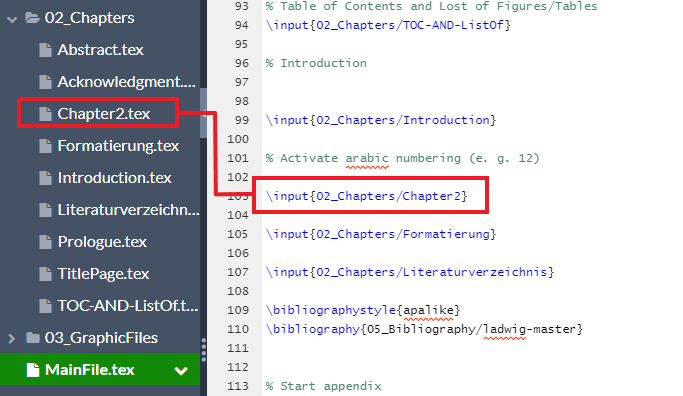
\includegraphics[width=\textwidth]{03_GraphicFiles/MainFile.png}
	\caption{Hier passende Caption einfügen}
	\label{fig:picture02}
\end{figure}

\begin{figure}[H]
	\centering  
	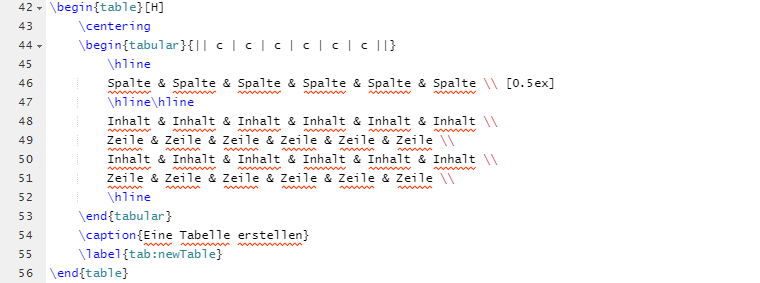
\includegraphics[width=\textwidth]{03_GraphicFiles/TabellenErstellen.PNG}
	\caption{Hier passende Caption einfügen}
	\label{fig:picture03}
\end{figure}

\newpage
\section{PDFs verlinken}\label{cha:pdfLink}
Es können auch bestimmte Seiten aus PDF-Dateien im Anhang dargestellt werden. Dazu muss man, wie bei Abbildungen, die gewünschte PDF in den passenden Ordner ablegen. Auf der folgenden Seite findet sich ein Ausschnitt aus dem Leitfaden für Masterarbeiten bei MIREVI.


\includepdf[pages={5}]{99_AppendixFiles/Leitfaden Abschlussarbeit.pdf}
